\section{Durchführung und Aufbau}
\label{sec:Durchführung}
Für den Versuch wird ein wie in Abbildung \ref{fig:Spek} zu sehendes Spektrometer benutzt.
\begin{figure}
  \centering
  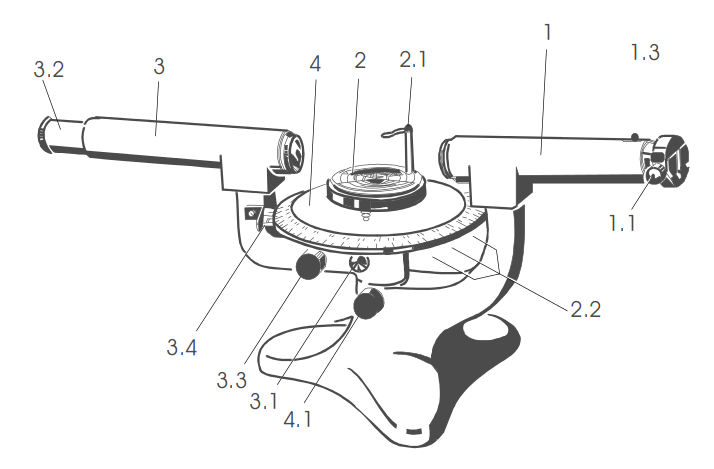
\includegraphics[height=5cm]{picture/Aufbau.png}
  \caption{Spektrometer ohne Leuchtmittel \cite{sample}}
  \label{fig:Spek}
\end{figure}
Vor das Spektrometer wird eine Alkali-Lampe gestellt so, dass das Licht durch die verstellbare Blende am Anfang des Spektrometers fällt. Anschließend wird das Licht im Kollomatorrohr gebündelt und am Gitter gebeugt. Mit dem Fernrohr werden die Beugungswinkel abgefahren und nach Maxima gesucht. Die von der Teilkreisplatte ablesbaren Winkel werden zu den entsprechenden Maxima notiert. Am Ende des Fernrohrs befindet sich desweiteren ein Okularmikrometer mit dem kleine Strecken ausgemessen werden können.

Zunächst wird die Heliumlampe vor das Spektrometer gestellt. Um im dem darauf folgenden Versuchsteil die Strecke $\Delta s$ der Dubletts zu vermessen wird zunächst das Okularmikrometer geeicht. Dafür wird die Stecke $\Delta t$ zweier bekannten Spektrallinien vermessen, anhand derer rückschlüsse auf die Skalierung des Okular gemacht werden kann. Mittels der Skalierung kann die Strecke $\Delta s$ zwischen den Dubletts berechnet werden. Ein Schema der Eichung ist in Abbildung \ref{fig:dup} zu sehen.
\begin{figure}
  \centering
  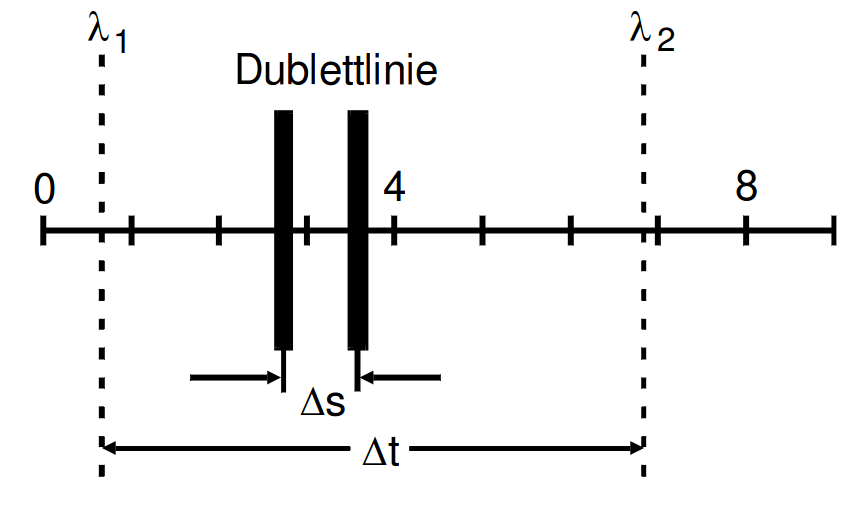
\includegraphics[height=6cm]{picture/Duplet.png}
  \caption{Messverfahren zur Bestimmung des Abstandes der Dublettlinien \cite{sample}}
  \label{fig:dup}
\end{figure}
Anschließend werden die Beugungswinkel $\varphi$ der verschiedenen Spektrallinien gemessen und notiert. Die Messung der Beugungswinkel wird für die Natrium-, Kalium- und Rubidiumlampen wiederholt. Desweiteren werden für diese Lampe die Strecken $\Delta s$ der Dubletts und deren Winkel vermessen. Für die Natriumlampe ist das rote, gelbe und grüngelbe Dublett zu vermessen.  Bei der Kaliumlampe sollen jeweils zwei gelbe und grüne Dubletts ausgemessen werden. Das Dublett der Rubidiumlampe, welches aus der dritten und vierten roten Spektrallinien besteht, soll ebenfalls vermessen werden.
